\documentclass{beamer}
%\documentclass[handout]{beamer}

\mode<handout>
{
  \usepackage{pgf}
  \usepackage{pgfpages}

\pgfpagesdeclarelayout{4 on 1 boxed}
{
  \edef\pgfpageoptionheight{\the\paperheight} 
  \edef\pgfpageoptionwidth{\the\paperwidth}
  \edef\pgfpageoptionborder{0pt}
}
{
  \pgfpagesphysicalpageoptions
  {%
    logical pages=4,%
    physical height=\pgfpageoptionheight,%
    physical width=\pgfpageoptionwidth%
  }
  \pgfpageslogicalpageoptions{1}
  {%
    border code=\pgfsetlinewidth{2pt}\pgfstroke,%
    border shrink=\pgfpageoptionborder,%
    resized width=.5\pgfphysicalwidth,%
    resized height=.5\pgfphysicalheight,%
    center=\pgfpoint{.25\pgfphysicalwidth}{.75\pgfphysicalheight}%
  }%
  \pgfpageslogicalpageoptions{2}
  {%
    border code=\pgfsetlinewidth{2pt}\pgfstroke,%
    border shrink=\pgfpageoptionborder,%
    resized width=.5\pgfphysicalwidth,%
    resized height=.5\pgfphysicalheight,%
    center=\pgfpoint{.75\pgfphysicalwidth}{.75\pgfphysicalheight}%
  }%
  \pgfpageslogicalpageoptions{3}
  {%
    border code=\pgfsetlinewidth{2pt}\pgfstroke,%
    border shrink=\pgfpageoptionborder,%
    resized width=.5\pgfphysicalwidth,%
    resized height=.5\pgfphysicalheight,%
    center=\pgfpoint{.25\pgfphysicalwidth}{.25\pgfphysicalheight}%
  }%
  \pgfpageslogicalpageoptions{4}
  {%
    border code=\pgfsetlinewidth{2pt}\pgfstroke,%
    border shrink=\pgfpageoptionborder,%
    resized width=.5\pgfphysicalwidth,%
    resized height=.5\pgfphysicalheight,%
    center=\pgfpoint{.75\pgfphysicalwidth}{.25\pgfphysicalheight}%
  }%
}


  \pgfpagesuselayout{4 on 1 boxed}[a4paper, border shrink=5mm, landscape]
  \nofiles
}
 % for handout 
%\setbeameroption{show notes} % uncomment to the the notes

\usepackage[T2A]{fontenc}
\usepackage[utf8]{inputenc}
\usepackage[russian]{babel}
\usepackage{amssymb,amsfonts,amsmath,mathtext}
\usepackage{cite,enumerate,float,indentfirst}
\usepackage[dvips]{graphicx}
\usepackage[linesnumbered,ruled,vlined]{algorithm2e} % NEW
\usepackage{algorithmic}
\usepackage{listings}

\lstset{
        breaklines=true,
        basicstyle=\footnotesize\ttfamily,
        prebreak =\raisebox{0ex}[0ex][0ex]{\ensuremath{\hookleftarrow}},
        postbreak =\raisebox{0ex}[0ex][0ex]{\ensuremath{\hookleftarrow}}
}

\setbeamertemplate{footline}[page number]

\title[\insertframenumber/\inserttotalframenumber]
{\textbf{Метрики семантической близости \\ с приложениями к задачам АОТ}}

\author[Александр Панченко]
{\textbf{Александр Панченко} \\ Université catholique de Louvain   \\ { \url{alexander.panchenko@uclouvain.be}  }}

\mode<presentation>
{
%\usetheme{Warsaw} % default beamer
%\usetheme{Singapore} % plain white
\usetheme{Luebeck}
\usecolortheme{default}
%\usecolortheme{orchid}% plain white
\useoutertheme{smoothbars}
%\usefonttheme{serif}
}


\setbeamertemplate{navigation symbols}{%
}

\AtBeginSubsection[]
{
	\begin{frame}<beamer>
  	\frametitle{План}
  	\tableofcontents[currentsection,currentsubsection,currentsubsubsection]
  	\end{frame}
}


\AtBeginSection[]
{
	\begin{frame}<beamer>
	\frametitle{План}
	\tableofcontents[currentsection]
	\end{frame}
}

\begin{document}

\begin{frame}
  \titlepage
\end{frame}

\begin{frame}
  \setcounter{tocdepth}{1}
  \frametitle{План}
  \tableofcontents
  \setcounter{tocdepth}{2}
	
\end{frame}

\section[Введение]{Введение}
\subsection{ }

\begin{frame}
\frametitle{Введение}

\begin{block}{Мотивация}

\begin{enumerate}
\item Метрики семантической близости \alert{полезны} для:
	\begin{itemize}
	\item систем обработки коротких текстов (Šaric et al., 2012; Panchenko at.,
	2012);
	\item расширешия поисковых запросов (Hsu et al., 2006);
	\item вопросно-ответных систем (Sun et al., 2005);
	\item разрешения омонимии (Patwardhan et al., 2003);
	\item \ldots 
	\end{itemize}

%\item Ручное создание семантических ресурсов непозволительно
%\alert{дорого}.
%\item  \alert{Качество} существующих систем извлечения недостаточно.
\end{enumerate}
\end{block}

\begin{itemize}
  \item Лексико-семантическое знание о языке.
  \item Вычислительная лексическая семантика.
  \item Computational Lexical Semantics. 
\end{itemize}

%\begin{block}{Focus}
%\alert{Similarity-based} semantic relation extraction.
%\end{block}

%\begin{block}{Research Question}
%How to \alert{improve} precision and coverage of such measures?
%\end{block}

\note[item]{\ldots}
\note[item]{\ldots}


\end{frame}







\begin{frame}
\frametitle{Метрики семантической близости}

\begin{block}{Определение}
  Метрика семантической близости численно выражает семантическую связность двух
  $c_i, c_j$: $s_{ij} =
  sim(c_i,c_j)$:
    $$
  s_{ij} = \left\{ 
   \begin{array}{l l}
    \text{велико} & \quad \text{если } \langle c_i, c_j \rangle \text{ -- пара }
    syn, hyper, cohypo \\
    0 & \quad \text{иначе}\\
   \end{array} \right.
 $$
 \end{block}


\begin{block}{Свойства}
\begin{itemize}    
  \item Неотрицательность: $0 \leq s_{ij} \leq 1$;
  \item Рефлективность: $s_{ij} = 1 \Leftrightarrow c_i = c_j$;
  \item Симметричность: $s_{ij} = s_{ji}$;
  \item $s_{ij} \leq s_{ik} + s_{kj}$  
  \end{itemize}
 \end{block}
     
\end{frame}




\begin{frame}
\frametitle{Метрики семантической близости}
\begin{itemize}

\item Малое количество подобных пар:
$s_{ij} \sim exp(\lambda)$.

\begin{figure}
\centering
\includegraphics[width=0.5\textwidth]{./../figures/reldist-crop}
\end{figure}

\item Распределение сем. близости слова ``doctor'':

\begin{figure}
\centering
\includegraphics[width=0.6\textwidth]{./../figures/real-extracted}
\end{figure} 

\end{itemize}
\end{frame}




\begin{frame}
\frametitle{Системы измерения семантической близости}
\begin{figure}
\centering
\includegraphics[width=0.9\textwidth]{./../figures/ssr-extraction-2}
\end{figure}
Как построить систему с высокой \textbf{точностью} и \textbf{лексическим покрытием}? 
\end{frame}





\begin{frame}
\frametitle{Оценка качества метрики семантической близости}

\begin{enumerate}
\item \textbf{Корреляция с суждениями человека о сем. близости}:
\begin{itemize}
  \item Статистики: корреляция Пирсона ($\rho$) и Спирмена ($r$).
  \item Проверочные данные: MC, RG, WordSim.
\end{itemize}

\item \textbf{Ранжирование семантических отношений}:
\begin{itemize}
  \item Точность, Полнота, F-мера.
  \item Проверочные данные: BLESS, SN.
\end{itemize}


\item \textbf{Точность извлечения семантических отношений:}
\begin{itemize}
  \item Статистики: Точность@k.
  \item Проверочные данные: аннотирование и/или тезаурусы.
\end{itemize}

\item \textbf{Использование метрики в системе АОТ:}
\begin{itemize}
\item в системе классификации имен файлов (\textbf{iCOP});
\item с системе поиска семантически связанных слов (\textbf{Serelex}).
\end{itemize}
\end{enumerate}


Panchenko A., \textbf{Similarity Measures for Semantic Relation Extraction.} PhD thesis. Universit\'{e} catholique de Louvain. 197 pages, 2013, (Chapter 1). 

\end{frame}



\section[Обзор метрик]{Обзор метрик семантической близости} 
\subsection{  }

\begin{frame}
\frametitle{Обзор метрик семантической близости}

\begin{figure}
\includegraphics[width=1.05\textwidth]{./../figures/measures-classification}
\end{figure}

\textbf{Публикации} (анализ 37 базовых метрик):
\begin{itemize}
\item Panchenko A., \textbf{Similarity Measures for Semantic Relation Extraction.} PhD thesis. Universit\'{e} catholique de Louvain. 197
pages, 2013, (Chapter 3). 
\item Panchenko A. \textbf{A Study of Heterogeneous Similarity Measures for Semantic Relation Extraction.} // In JEP-TALN-RECITAL 2012 — Grenoble (France), 2012. 
\end{itemize}
 
\end{frame}



%%%%%%%%%%%%%%%%%%%%%%%%%%%%%%%%%%%%%%%%%%%%%%%%%
\begin{frame}
\frametitle{Метрики основанные на семантической сети}

 \textbf{Данные:} семантическая сеть WordNet 3.0, корпус SemCor.
	
 \textbf{Переменные:}
\begin{itemize}
\item $len(c_i,c_j)$ -- длина \textbf{кратчайшего пути} между $c_i$ и $c_j$
\item  $len(c_i, lcs(c_i,c_j))$ -- длина кратчайшего пути от $c_i$ до \textbf{ближайшего общего предка  (БОП)} слов $c_i$ и $c_j$
\item $len(c_{root}, lcs(c_i,c_j))$ -- длина кратчайшего пути от \textbf{корня} $c_{root}$ до БОП слов $c_i$ и $c_j$ (глубина БОП)
\item $P(c)$ --  \textbf{вероятность слова} $c$, оцененная из корпуса
\item  $P(lcs(c_i, c_j))$ -- \textbf{вероятность БОП} слов $c_i$ и $c_j$
\end{itemize}
	
 \textbf{Метрики:} Инвертированная длина пути (Jurafsky and Martin, 2009), Leacock-Chodorow (1998), Wu-Palmer (1994), 
 Resnik (1995), Jiang-Conrath (1997), Lin (1998).
  
\end{frame}

%%%%%%%%%%%%%%%%%%%%%%%%%%%%%%%%%%%%%%%%%%%%%%%%%
\begin{frame}
\frametitle{Метрики основанные на Веб корпусе текстов }

\textbf{Данные:} количество документов возвращенных ИПС: Google, 
Yahoo, AltaVista, Bing, и т.п.
	
\textbf{Переменные:} 
\begin{itemize}
	\item $h_i$ -- \textbf{количество документов} возвращенных по запросу слова
	$"c_i"$
	\item $h_{ij}$ -- \textbf{количество документов} возвращенных по запросу $"c_i \text{ AND } c_j"$
\end{itemize}

\textbf{Метрики:} 
\begin{itemize}
\item Normalized Google Distance (NGD) (Cilibrasi and Vitanyi, 2007)
\item Pointwise Mutual Information - Information Retrieval (PMI-IR) (Turney,
2001)
\end{itemize}
\end{frame}

%%%%%%%%%%%%%%%%%%%%%%%%%%%%%%%%%%%%%%%%%%%%%%%%%
\begin{frame}
\frametitle{Дистрибутивные метрики}


\textbf{Данные:} корпус, такой как Википедия или ukWaC

	
\textbf{Переменные:} 
\begin{itemize}
  \item $\textbf{f}_i$-- вектор признаков представляющий слово $c_i$, основанный на \textbf{контекстном окне}
  \item $ \mathbf{f}^s_i$ -- вектор признаков представляющий слово $c_i$, основанный на \textbf{синтаксическом контекстном окне}
  \begin{figure}
         \centering
         \includegraphics[width=0.9\textwidth]{./../figures/10-figure-3-gray}
         %\caption{ Representing the descriptor ``proposition de loi'' with
         %syntactic features coming from the dependency parser XIP. }
 \end{figure}
   
\end{itemize}
	
\textbf{Метрики:}
\begin{itemize}
	\item Bag-of-words Distributional Analysis (BDA) (Sahlgren, 2006)
	\item Syntactic Distributional Analysis (SDA) (Curran, 2003)
\end{itemize}	
\end{frame}
	





\begin{frame}
\frametitle{Другие метрики основанные на корпусе текстов}

\textbf{Данные:} корпус, такой как Википедия или ukWaC
	
	
\textbf{Метрики:}
\begin{itemize}	
\item Латентно-cемантический анализ (LSA) (Landauer and Dumais, 1997)
\item Вероятностные модели (pLSA, LDA и др.) (Griffiths et al., 2007)
\item NGD и PMI-IR (Veksler et al., 2008)
\item \ldots
\end{itemize}
	
\end{frame}



%%%%%%%%%%%%%%%%%%%%%%%%%%%%%%%%%%%%%%%%%%%%%%%%%
\begin{frame}
\frametitle{Метрики основанные на определениях}

\textbf{Данные:} определения из WordNet, Википедии, Викисловаря или любого
другого словаря.
	
\textbf{Переменные:}
\begin{itemize}
		\item $gloss(c_i)$ -- \textbf{определение} слова $c_i$;
		\item $\mathbf{f}_i$ \textbf{вектор признаков}, построенный из $gloss(c_i)$;
		\item $\mathbf{f}_i$ -- \textbf{вектор признаков} $c_i$, вычисленный на
		корпусе из всех определений методом контекстного окна;
		
		\item $exist(c_i, c_j)$ -- наличие связи между $c_i$ и $c_j$ в словаре.
\end{itemize}

\textbf{Метрики:}
\begin{itemize}
  \item ExtendedLesk (Banerjee and Pedersen, 2003)
  \item GlossVectors (Patwardhan and Pedersen, 2006)
  \item DefVectors (Панченкo и др., 2012), (Panchenko et al., 2012)
  
\end{itemize}

\end{frame}




\begin{frame}
\frametitle{Лучшие базовые метрики семантической близости}

\begin{figure}
\includegraphics[width=1.05\textwidth]{./../figures/best}

\end{figure}

\begin{itemize}
  \item Каждая метрика излекает много \alert{ко-гипонимов}: 
  \begin{itemize}
  \item $\langle Canon, Nikon \rangle$,
  \item $\langle Lamborghini, Ferrari \rangle$,
  \item $\langle Obama, Romney \rangle$.
\end{itemize}
\end{itemize}
   
\end{frame}





\begin{frame}
\frametitle{Резюме}

\begin{block}{Основные ресурсы для построения метрик:}
\begin{itemize}
  \item семантические сети и тезаурусы;
  \item корпуса текстов;
  \item Веб корпус текстов;
  \item определения из словарей и энциклопедий. 
\end{itemize}
\end{block}   


\begin{block}{Метрики \textbf{дополняют друг друга} в терминах:}
\begin{itemize}
  \item лексического покрытия;
  \item точности;
  \item типов извлекаемых отношений. 
\end{itemize}
\end{block}   

\end{frame}





\begin{frame}
\frametitle{Программное обеспечение}

\begin{itemize}
  \item \textbf{Semantic Vectors:} \url{https://code.google.com/p/semanticvectors/}
  \item \textbf{S-Space Package:} \url{https://code.google.com/p/airhead-research/}
  \item \textbf{WordNet::Similarity:} \url{http://wn-similarity.sourceforge.net}
  \item \textbf{NLTK:} \url{http://nltk.googlecode.com/svn/trunk/doc/howto/wordnet.html}
  \item \textbf{WikiRelate!}
  \item \textbf{PatternSim / Serelex:} \url{http://serelex.cental.be}
  \item \textbf{Метрики основанные на Веб корпусе:} \url{http://cwl-projects.cogsci.rpi.edu/msr}
  \item \textbf{LSA:} \url{http://lsa.colorado.edu}
  \item \textbf{DefVectors:} \url{http://github.com/jgc128/defvectors}
\end{itemize}

\end{frame}

   
\section[PatternSim]{Метрика основанная на лексико-синтаксических шаблонах}

\subsection{}

\begin{frame}
\frametitle{Публикации}

\begin{itemize}
\item Panchenko A., Morozova O., Naets H. \textbf{A Semantic Similarity Measure Based on Lexico-Syntactic Patterns.} In Proceedings of KONVENS 2012, pp.174--178, 2012
\item Panchenko A., Romanov P., Morozova O., Naets H., Philippovich A., Fairon
C. \textbf{Serelex: Search and Visualization of Semantically Related Words}.
In Proceedings of the 35th European Conference on Information Retrieva (ECIR 2013).

\item Панченко А., Романов П., Романов А.,  Филиппович А.,
Филиппович Ю., Морозова О. \textbf{Серелекс: поиск и визуализация
семантически связанных слов}. (АИСТ 2013)
\end{itemize}
\end{frame}

\begin{frame}
\frametitle{Демо}

\begin{itemize}
  \item {\bf \url{http://serelex.cental.be/} }
  
\begin{figure}	
	\centering
		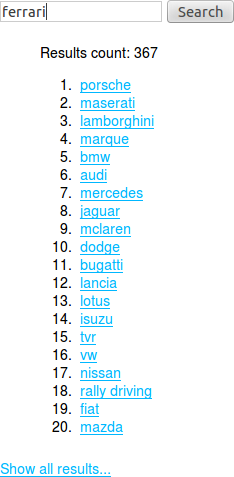
\includegraphics[height=0.6\textwidth]{figures/serelex}
		
\includegraphics[height=0.5\textwidth]{figures/spacer}
		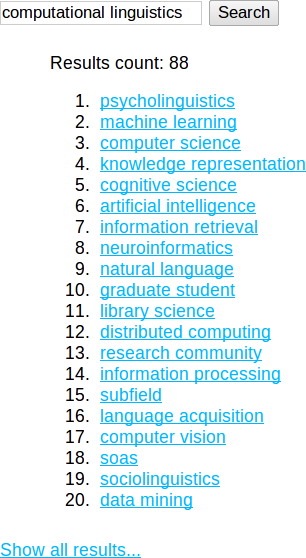
\includegraphics[height=0.6\textwidth]{figures/serelex-2}
		\end{figure}
\end{itemize}
\end{frame}


\begin{frame}
\frametitle{Лексико-синтаксические паттерны}

\begin{itemize}
  \item 18 паттернов извлекающих \textbf{гиперонимы},
  \textbf{ко-гипонимы} и \textbf{синонимы}
\begin{figure}	
	\centering
		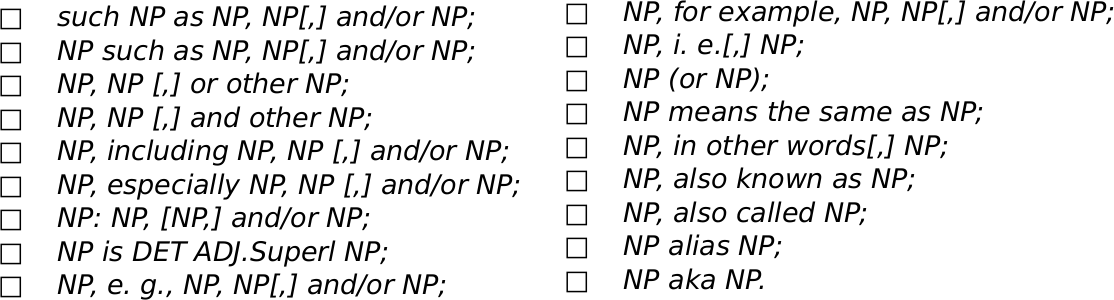
\includegraphics[width=1.0\textwidth]{figures/patterns}
	\end{figure}
\end{itemize}

\end{frame}

\begin{frame}
\frametitle{Основной каскад автоматов}

\begin{itemize}
  \item Каскад конечных автоматов (FST)
  \item В формете \texttt{Unitex}
\begin{figure}	
	\centering
		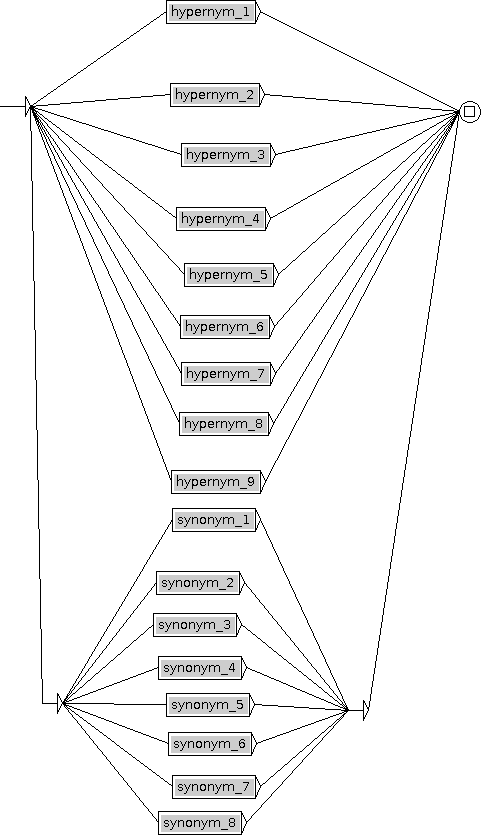
\includegraphics[width=0.3\textwidth]{figures/main-graph}
	\end{figure}
\end{itemize}

\end{frame}

\begin{frame}
\frametitle{Пример реализации паттерна в виде автомата}

\begin{figure}	
	\centering
		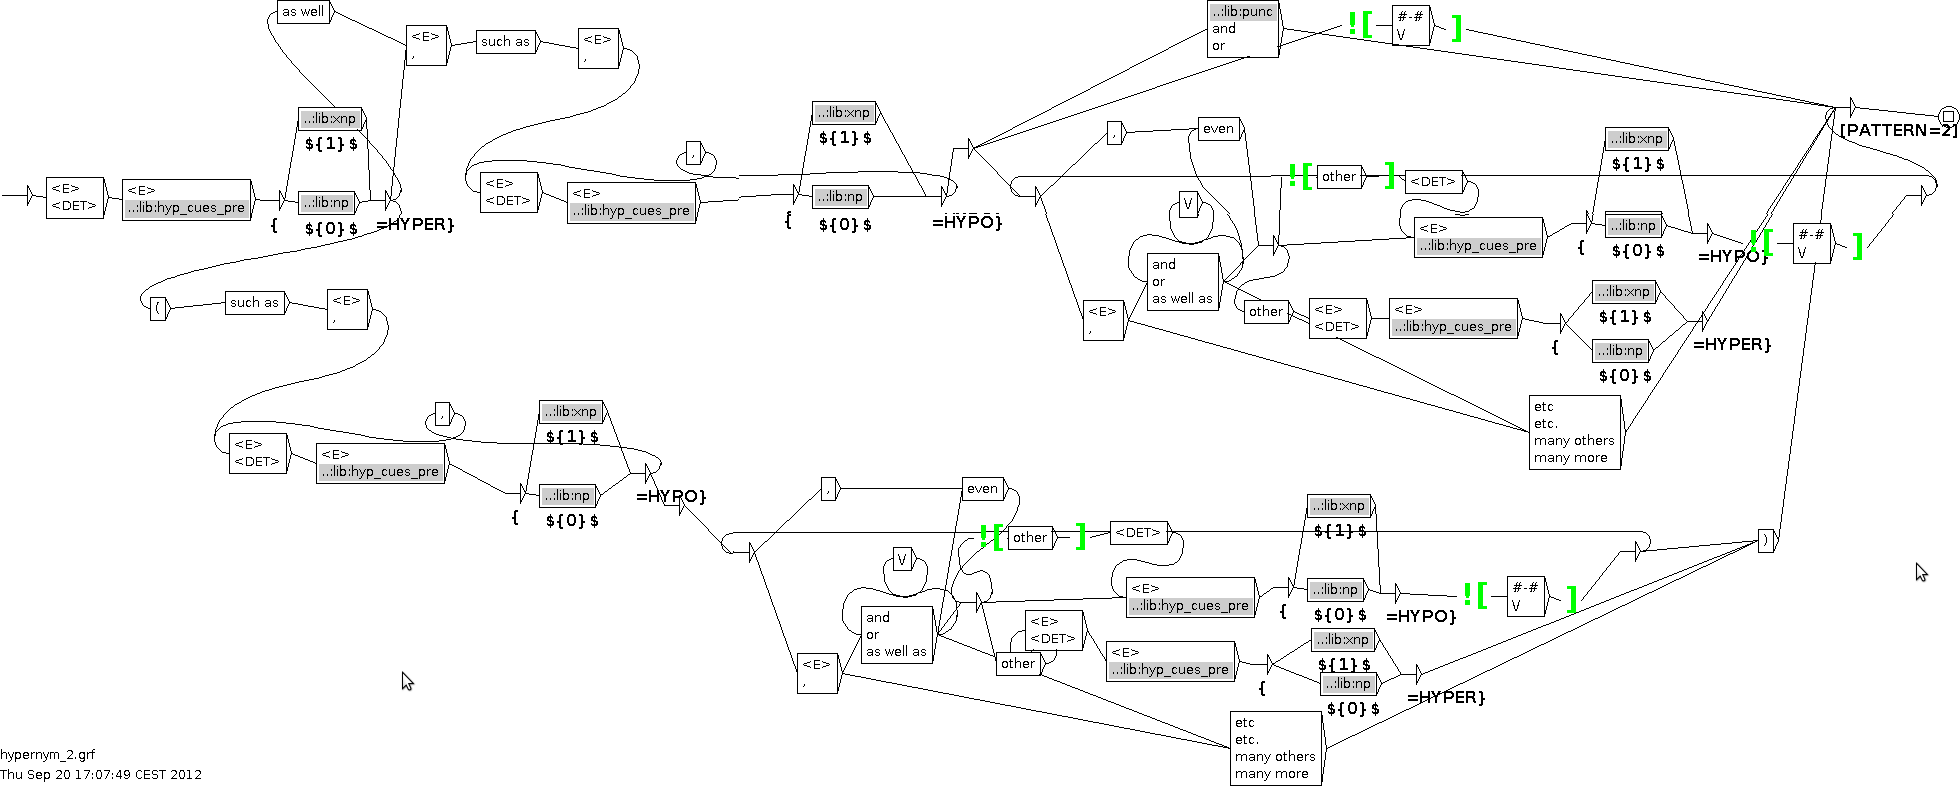
\includegraphics[width=1.0\textwidth]{figures/pattern2}
	\end{figure}

\begin{itemize}
  \item Паттерны основанные на автоматах позволяют учесть лингвистическую вариацию сохраняя
  точность
	  \item В отличие от паттернов основанных на строках (Bollegala et al., 2007)
	
\end{itemize}

\end{frame}





\begin{frame}
\frametitle{PatternSim: основные этапы}

\textbf{Корпус} Wikipedia+ukWaC: $2.9\cdot10^{12}$ токенов

\textbf{Паттерны извлекают конкордансы}

\begin{itemize}
  \item \texttt{such diverse \{[occupations]\} as
  \{[doctors]\}, \{[engineers]\} and \{[scientists]\}[PATTERN=1]}
  \item \texttt{such \{non-alcoholic [sodas]\} as \{[root beer]\} and \{[cream soda]\}[PATTERN=1]}
  \item \texttt{\{traditional[food]\}, such as \{[sandwich]\},\{[burger]\}, and \{[fry]\}[PATTERN=2]}
\end{itemize}

\textbf{Количество извлечений}

\begin{itemize}
  \item Wikipedia -- 1.196.468 
  \item ukWaC -- 2.227.025 
  \item WaCypedia+ukWaC -- 3.423.493
\end{itemize}

\textbf{Вычисление подобия}

\end{frame}




\begin{frame}
\frametitle{Формула Efreq-Rnum-Cfreq-Pnum}

  
$$s_{ij} = \sqrt{p_{ij}} \cdot \frac{2\cdot\mu_b }{b_{i*}+b_{*j}} \cdot \frac{P(c_i,c_j)}{P(c_i)P(c_j)}.$$


\begin{itemize}

%\item $s_{ij}$ -- semantic similarity between terms $c_i, c_j \in C$

\item $P(c_i,c_j)=\frac{e_{ij}}{\sum_{ij}e_{ij}}$ -- вероятность извлечения
отношения $\langle c_i,c_j \rangle$, где $e_{ij}$ -- частота
взаимной встречаемости слов $c_i$ и $c_j$ во множестве конкордансов

\item $P(c_i)= \frac{f_i}{\sum_i f_i}$ -- вероятность слова $c_i$, где $f_i$
-- частота $c_i$
\item $b_{i*} = \sum_{j:e_{ij} \geq \beta} 1$ -- количество извлечений слова
$c_i$ с частотой $\geq \beta$,  где $\mu_b = \frac{1}{|C|}\sum_{i=1}^{|C|}
b_{i*}$ -- среднее количество извлечений для отдельного слова

\item $p_{ij} \in [1;18]$ -- количество отдельных паттернов которые извлекли
отношение $\langle c_i, c_j \rangle$
  
 
\end{itemize}

\end{frame}






\begin{frame}
\frametitle{Ранжирование семантических отношений}

\begin{itemize}
  \item Точность \textbf{сравнима или лучше} чем у аналогов;
  \item Полнота \textbf{меньше} чем у аналогов.
\end{itemize}

\begin{figure}	
	\centering
	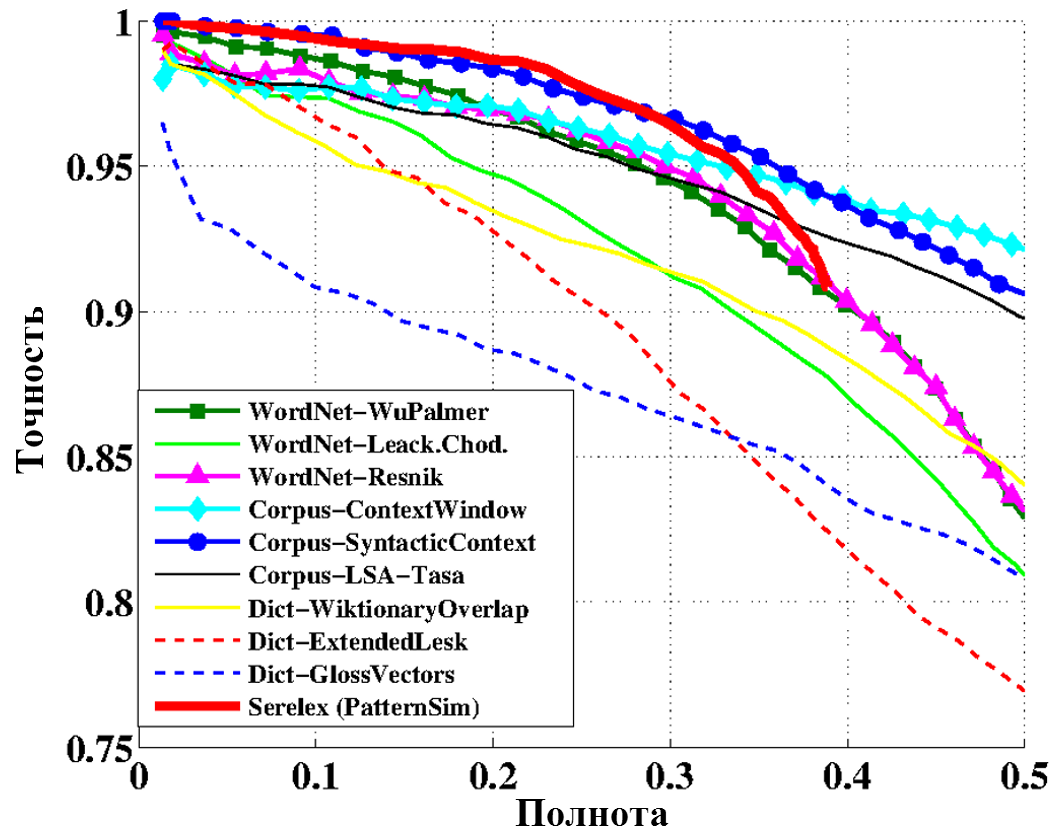
\includegraphics[width=0.6\textwidth]{pr}
	\caption{График точность-полнота (коллекция BLESS).
	}
\end{figure}

\end{frame}





\begin{frame}
\frametitle{Извлечение семантических отношений}
  \begin{columns}[T]
    \begin{column}{.4\textwidth}
     
% Your text here
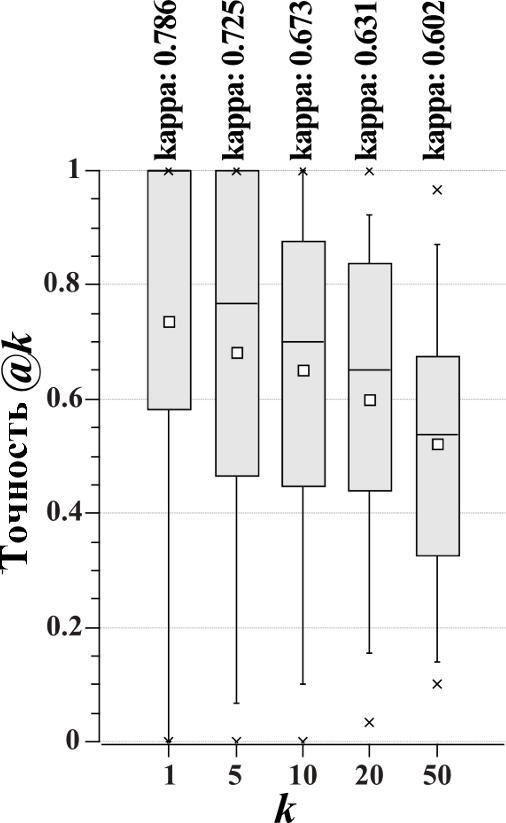
\includegraphics[width=0.85\textwidth]{./kappa}
    
    \end{column}
    \begin{column}{.6\textwidth}
    %\begin{block}{Your image}
\begin{itemize}
  %\item 49 words, three binary annotations;
  \item Точность@1 $\approx 0.80$;
  \item ``Хорошее'' лексическое покрытие:
  
\end{itemize}

\begin{figure}
\includegraphics[width=0.95\textwidth]{./../figures/wordnet-vs-serelex}
\end{figure}
      
    \end{column}
  \end{columns}
\end{frame}












%%%%%%%%%%%%%%%%%%%%%%%%%%%%%%%%%%%%%%%%%%%%%%%%%
\section[HybridSim]{Гибридная метрика семантической близости}

\subsection{}

\begin{frame}
\frametitle{Публикациии}
\begin{itemize}
\item Panchenko A., Morozova O. \textbf{A Study of Hybrid Similarity Measures
for Semantic Relation Extraction.} // Innovative Hybrid Approaches to the Processing of Textual Data Workshop, EACL 2012 — Avignon (France), 2012 — pp. 10–18 
\item Panchenko A., \textbf{Similarity Measures for Semantic Relation
Extraction.} PhD thesis. Universit\'{e} catholique de Louvain. 197
pages, 2013, (Chapter 4). 

\item Panchenko A. \textbf{A Study of Heterogeneous Similarity Measures for
Semantic Relation Extraction.} // In JEP-TALN-RECITAL 2012 — Grenoble (France), 2012 — pp. 29–42.
\end{itemize}
\end{frame}


%### A multitude of \textbf{complimentary measures} were proposed to extract synonyms, hypernyms,
%and co-hyponyms

%### Most of them are based on \textbf{one} of the \textbf{5 key approaches}: 
%\begin{enumerate}
%\item distributional analysis (Lin, 1998b)
%\item web as a corpus (Cilibrasi and Vitanyi, 2007)
%\item lexico-syntactic patterns (Bollegala et al., 2007)
%\item semantic networks (Resnik, 1995)
%\item definitions of dictionaries or encyclopedias (Zesch et al., 2008a)
%\end{enumerate}

%\item Some attempts were made to \textbf{combine measures} (Curran, 2002; Cederberg and Widdows, 2003; Mihalcea et al., 2006;
%Agirre et al., 2009; Yang and Callan, 2009)

%### \item However, most studies are still \textbf{not taking into account} all 5 existing extraction approaches.


\begin{frame}
\frametitle{Отдельные и гибридные метрики}

\begin{figure}
\centering
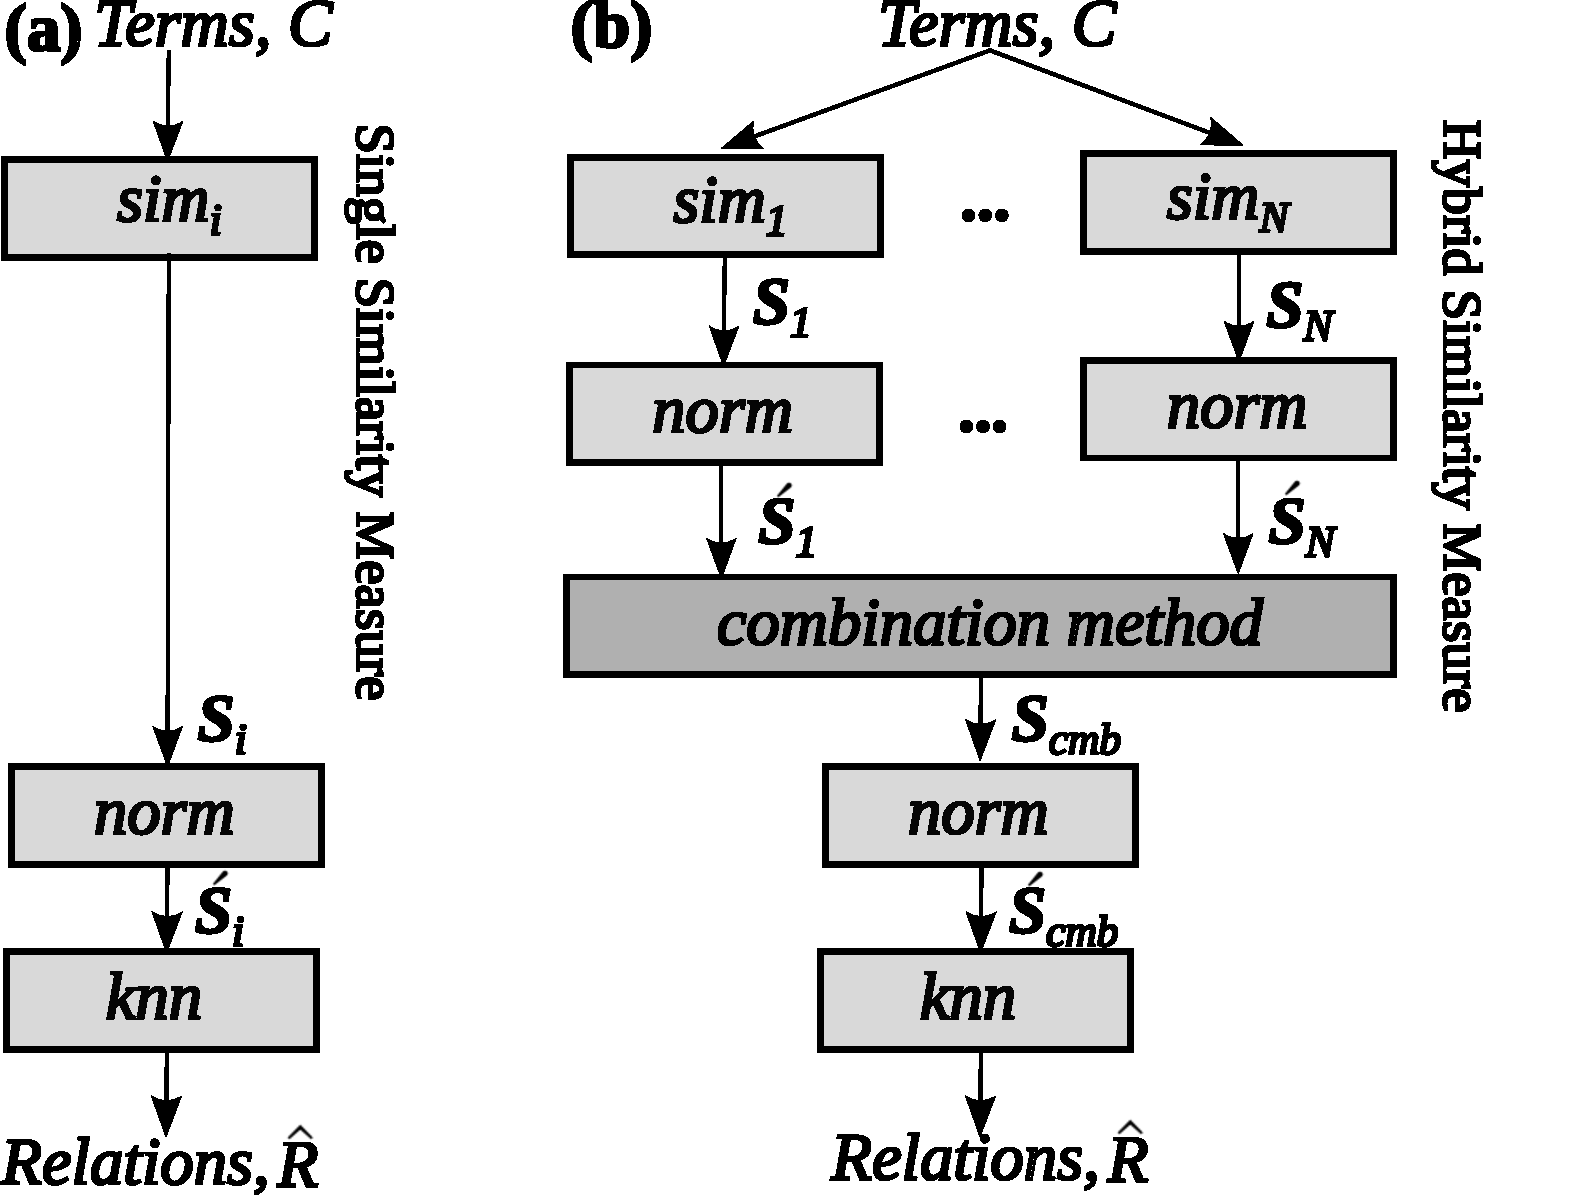
\includegraphics[width=0.65\textwidth]{./../figures/papers/4/src/figures/single-and-hybrid-2}
\caption{Система извлечения семантических отношений основанная на:
\begin{itemize}
\item \textbf{(a)} \textbf{отдельной} метрике;
\item \textbf{(b)} \textbf{гибридной} метрике. 
\end{itemize}}
\end{figure}
\end{frame}





\begin{frame}
\frametitle{16 признаков = 16 отдельных метрик}

	\begin{itemize}
	
	\item 5 метрик основанных на \textbf{семантических сетях}:
	\begin{enumerate}
	  \item WuPalmer;
	  \item Leacock and Chodorow;
	  \item Resnik;
	  \item Jiang and Conrath;
	  \item Lin.
	\end{enumerate} 
	\item 3 метрики основанных на \textbf{Веб корпусе} (NGD-Yahoo/Bing/Google);
		
	\item 5 метрики основанные на \textbf{корпусе текстов}: 
	\begin{itemize}
	  \item 2 дистрибутивных (BDA, SDA)
	  \item 1 лексико-синтаксические шаблоны (PatternSim)
	  \item 2 другие (LSA, NGD-Factiva)
	\end{itemize}
	
	\item 3 метрики основанные на \textbf{определениях} 
	\begin{enumerate}
	  \item ExtendedLesk;
	  \item GlossVectors;
	  \item DefVectors-WktWiki.
	\end{enumerate}
	 
\end{itemize}

\end{frame}


%\begin{frame}
%\frametitle{Способы комбинирования без учителя}

%\begin{enumerate}
  
%a mean of $K$ pairwise similarity scores;
%\item \textbf{Mean}: $s_{ij}^{cmb}= \frac{1}{K}\sum_{k=1,K} s_{ij}^k;$

%-- a mean of scores having non-zero value;
%\item \textbf{Mean-Nnz}: $s_{ij}^{cmb}= \frac{1}{|k:s_{ij}^k >0,k=1,K|}\sum_{k=1,K} s_{ij}^k;$ 

%-- A mean of scores transformed into Z-scores;
%\item \textbf{Mean-Zscore}: $\mathbf{S}_{cmb} = \frac{1}{K} \sum_{k=1}^K \frac{\mathbf{S}_k -
%\mu_k}{\sigma_k};$

% where $\mu_k$ and $\sigma_k$ are a mean and a standard deviation of the scores of the $k$-th measure ($\mathbf{S}_k$).

%. A median of $K$ pairwise similarities:
%\item \textbf{Median}: $s_{ij}^{cmb}= median(s_{ij}^1,\ldots,s_{ij}^K);$

% A maximum of $K$ pairwise similarities:
%\item \textbf{Max}: $s_{ij}^{cmb}= max(s_{ij}^1,\ldots,s_{ij}^K);$

%A mean of scores converted to ranks:
%\item \textbf{RankFusion}: $s_{ij}^{cmb}= \frac{1}{K}\sum_{k=1,K} r_{ij}^k;$

%where  $r^k_{ij}$ is the rank corresponding to the similarity score $s^k_{ij}$.
%\item \textbf{RelationFusion} (Panchenko and Morozova, 2012).
%\end{enumerate}

%\end{frame}





\begin{frame}
\frametitle{Методы комбинирования}

\begin{enumerate}
  \setcounter{enumi}{7}
\item \textbf{Logit}, \textbf{Logit-L1}, \textbf{Logit-L2}. 

\begin{itemize}
  \item  Бинарная \textbf{логистическая регрессия};

\item \textbf{Положительные обучающие примеры} -- синонимы, гиперонимы,
ко-гипонимы из BLESS/SN;
\item \textbf{Отрицательные обучающие примеры} -- случайные пары семантически
несвязных слов из BLESS/SN;

  \item Отношение $\langle c_i,t, c_j \rangle \in R$ представлено с помощью
  \textbf{вектора попарных близостей}: $\mathbf{x} = (s_{ij}^1,\ldots,s_{ij}^N),
  N=\overline{2,16}$;

\item Категория $y_{ij}$:
$$
y_{ij} = \left\{ 
  \begin{array}{l l}
    0 & \quad  \text{ если } \langle c_i,t, c_j \rangle \text{ случайное
    отношение}
    \\
    1 & \quad  \text{ иначе }\\
  \end{array} \right
  .
$$

\item \textbf{Использование модели} $(w_1,\ldots,w_K)$ для комбинирования: 
$$s^{cmb}_{ij} = \frac{1}{1 + e^{-z}}, z = \sum_{k=1}^K w_k s^k_{ij} + w_0.$$

\end{itemize}
\end{enumerate}

\end{frame}



\begin{frame}
\frametitle{Методы комбинирования}

\begin{enumerate}
  \setcounter{enumi}{8}
\item \textbf{SVM}. 


\begin{columns}
  \begin{column}{0.5\textwidth}
\begin{figure}
\centering
\includegraphics[width=1.0\textwidth]{./../figures/svm}
%\caption{SVM: maximal margin hyperplane. }
\end{figure}
    
  \end{column}

  \begin{column}{0.5\textwidth}
\begin{itemize}
\item Веса $\mathbf{w}$ и опорные вектора $SV$: 

$$
\mathbf{w} = \sum_{x_i \in SV} \alpha_i y_i \mathbf{x}_i.  
$$

\item \textbf{Использование модели} 

$$
s_{ij}^{cmb} = \mathbf{w}^T\mathbf{x} + b = \sum_{k=1}^K w_i s_{ij}^k + b.
$$

\end{itemize}    
  \end{column}
\end{columns}





\end{enumerate}

\end{frame}









\begin{frame}
\frametitle{Методы комбинирования с учителем}
\begin{figure}
\centering
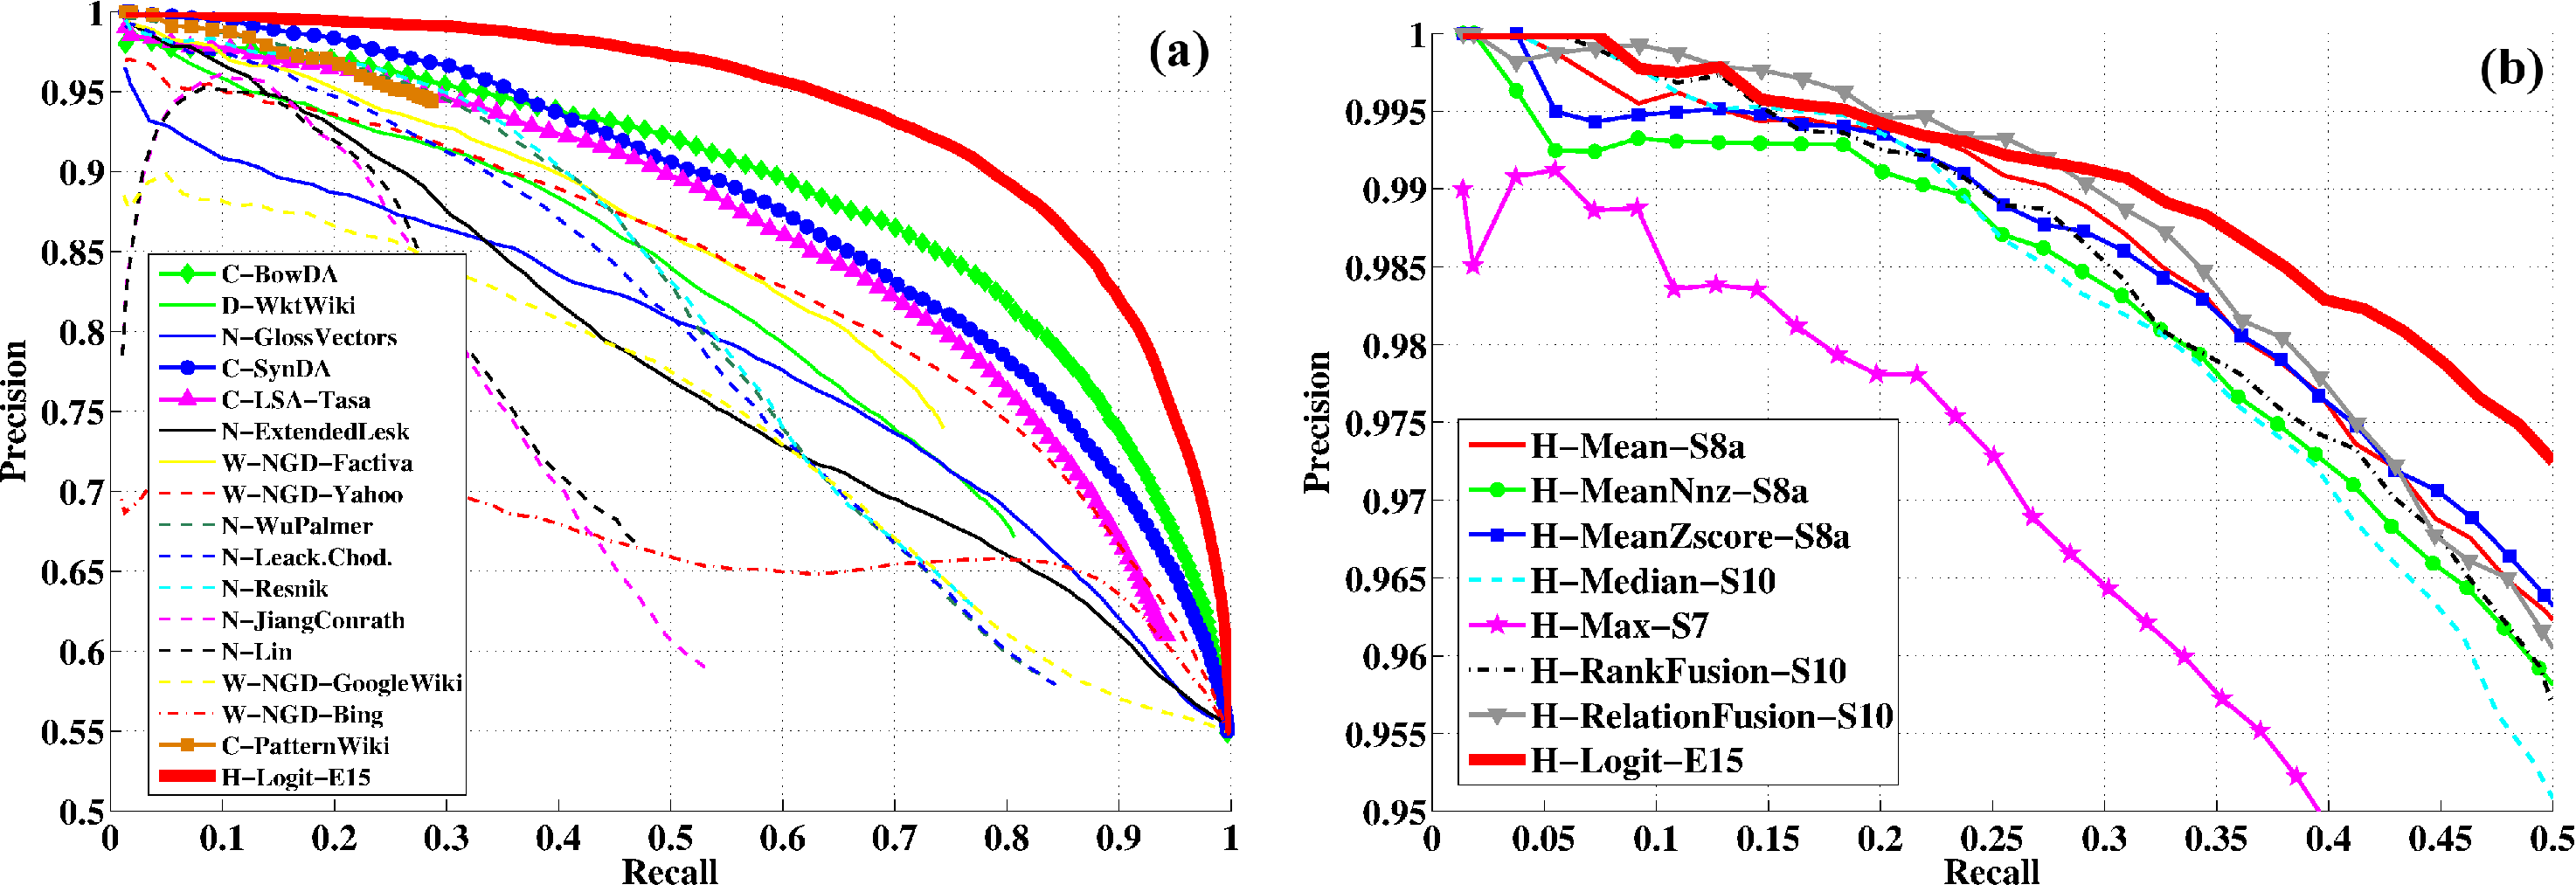
\includegraphics[width=1.0\textwidth]{figures/pr}
%\caption{

%}
\end{figure}

График Точность-Полнота вычисленный на коллекции BLESS:
\begin{itemize}
  \item \textbf{(a)} 16 отдельных метрик и гибридная метрика Logit-E15;
  \item \textbf{(b)} 8 гибридных метрик.
\end{itemize}

\end{frame}



\begin{frame}
\frametitle{Методы комбинирования с учителем Logit-E15}
\begin{figure}
\centering
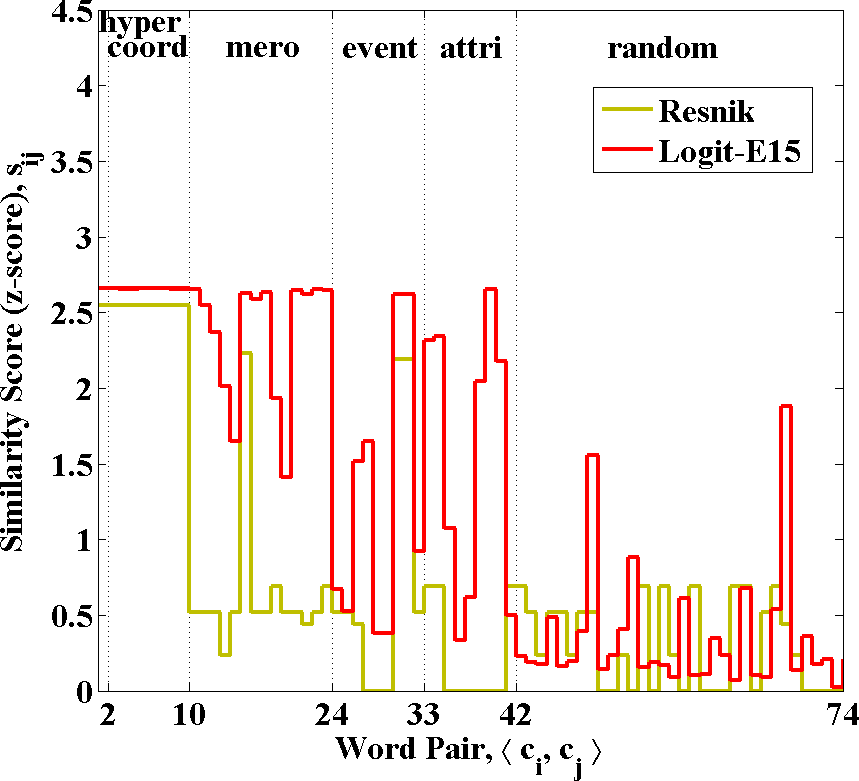
\includegraphics[width=0.30\textwidth]{figures/acacia-resnik} 
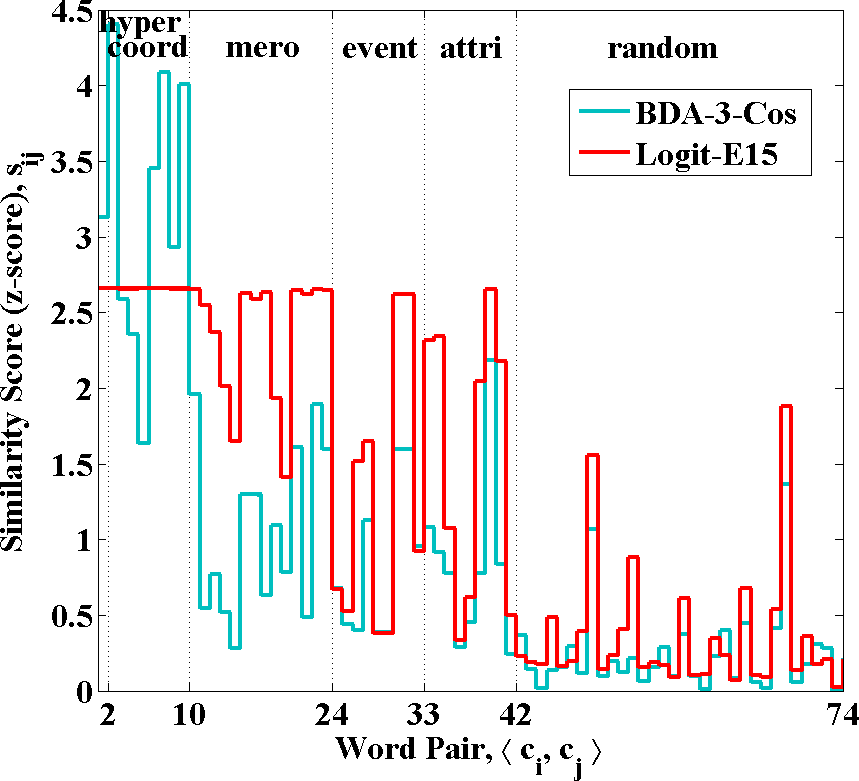
\includegraphics[width=0.30\textwidth]{figures/acacia-bda}
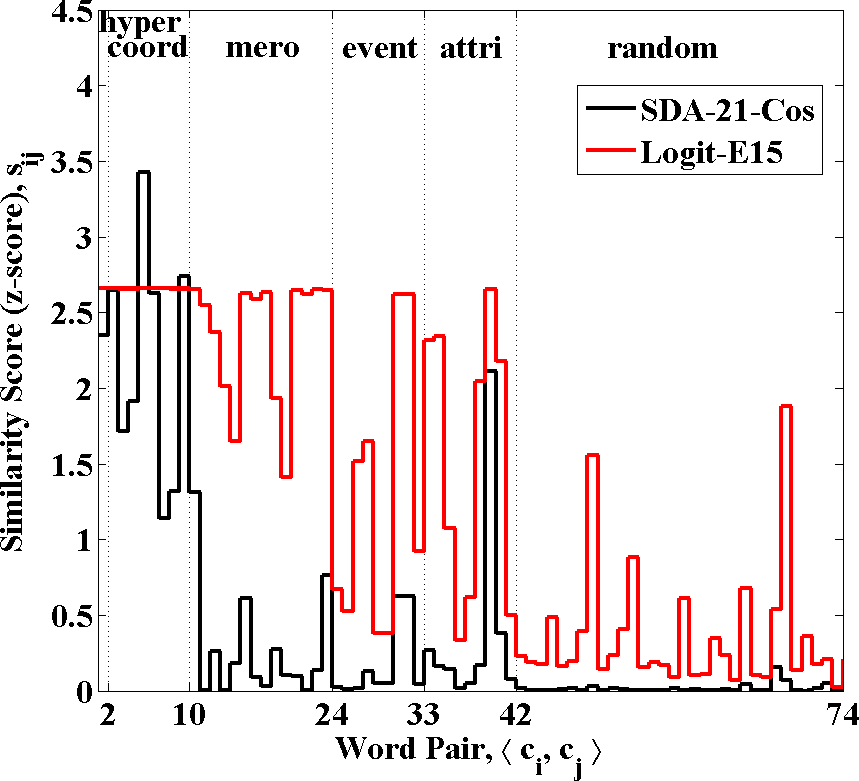
\includegraphics[width=0.30\textwidth]{figures/acacia-sda}

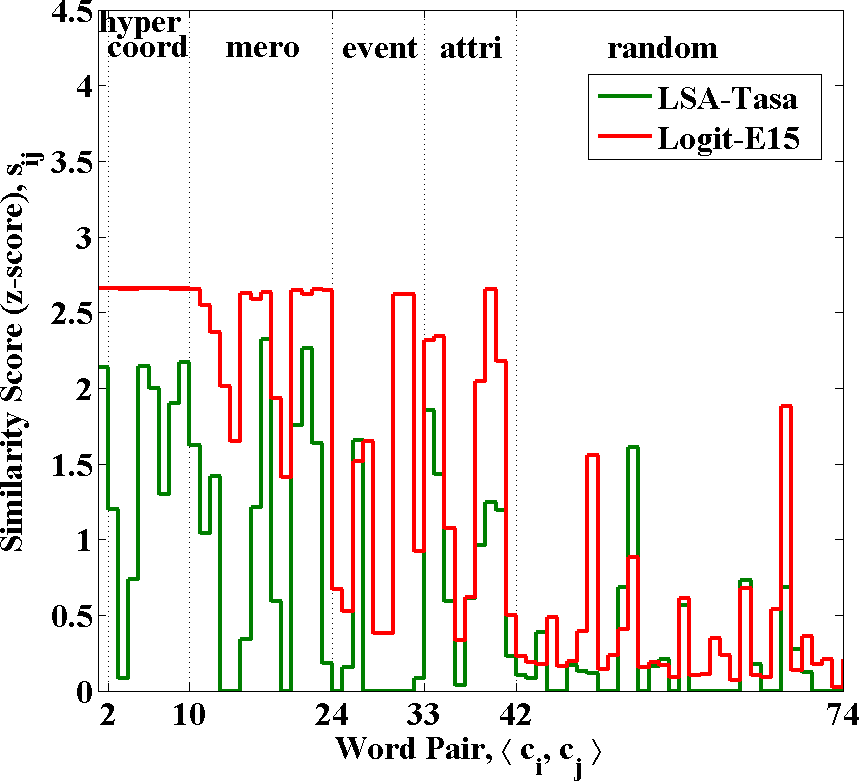
\includegraphics[width=0.30\textwidth]{figures/acacia-lsa}
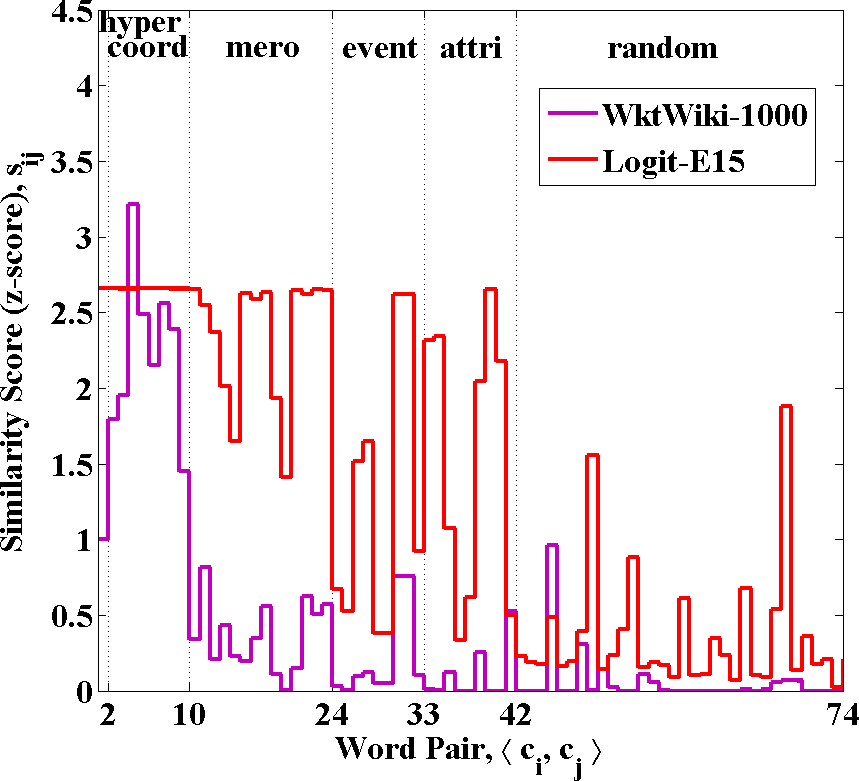
\includegraphics[width=0.30\textwidth]{figures/acacia-ww}
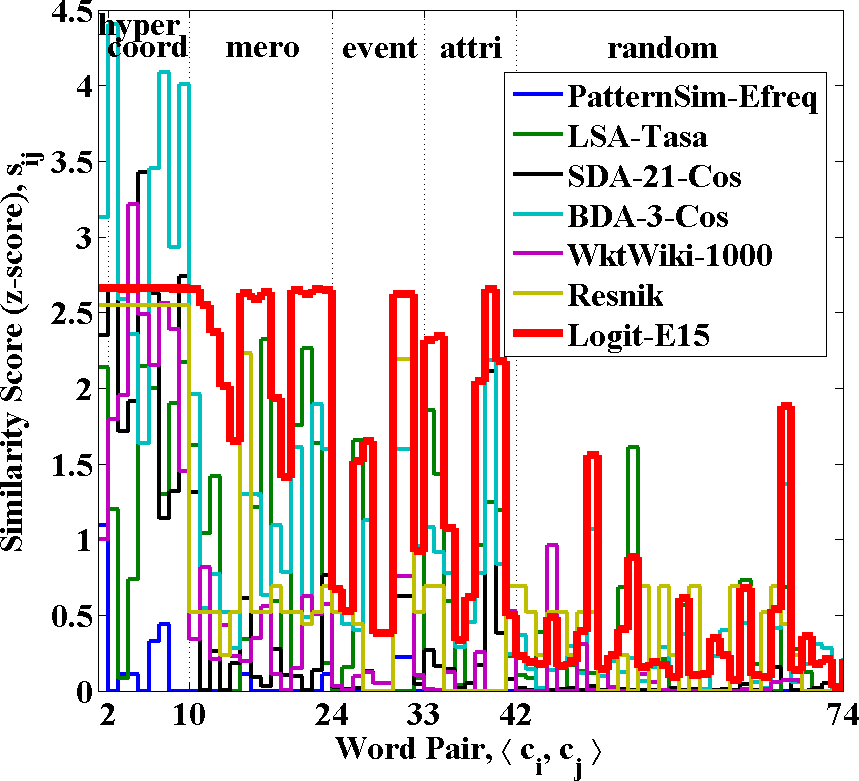
\includegraphics[width=0.30\textwidth]{figures/acacia}
\caption{ Значение подобия между 74 словами связанными со словом ``acacia''.
}
\label{fig:hybrid-complimentary-discussion}
\end{figure}

\end{frame}


\begin{frame}
\frametitle{Методы комбинирования с учителем}

	\begin{figure}
	\centering
		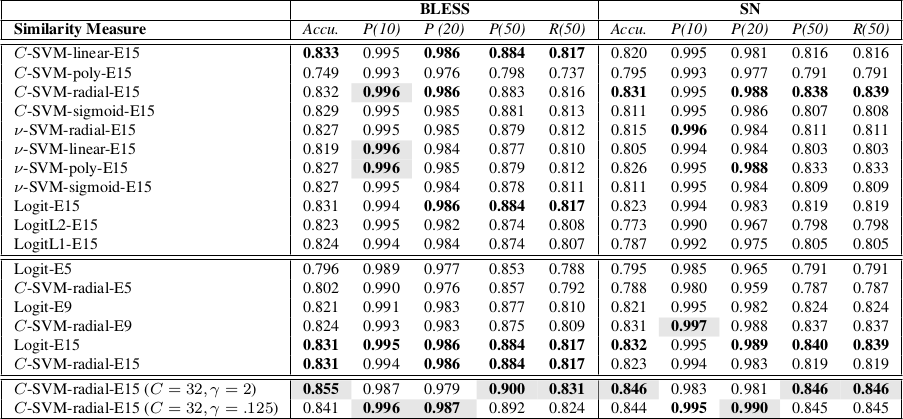
\includegraphics[width=1.0\textwidth]{figures/hybrid-table}
		
		%\caption{ Performance of the hybrid supervised semantic similarity measures. }
\end{figure}
\end{frame}


\begin{frame}
\frametitle{Методы комбинирования с учителем (продолжение)}
\begin{figure}
\centering
\includegraphics[height=0.4\textwidth]{./../figures/sn-accuracy}
\includegraphics[height=0.4\textwidth]{./../figures/bless-accuracy}
%
\includegraphics[height=0.025\textwidth]{./../figures/spacer}
%\includegraphics[height=0.36\textwidth]{./../figures/bless-precision10}
%\includegraphics[height=0.36\textwidth]{./../figures/bless-precision20}
%
\includegraphics[height=0.025\textwidth]{./../figures/spacer}
%\includegraphics[height=0.36\textwidth]{figures/bless-precision50}
%\includegraphics[height=0.36\textwidth]{figures/bless-recall50}     
     
\caption{ Оптимизация мета-параметров метрики C-SVM-radial-E15.  }
\label{fig:radial-optimization}
\end{figure}
\end{frame}


\section[Приложения]{Приложения метрик семантической близости}
\subsection{Поиск и визуализация семантически связанных слов}

  


\begin{frame}
\frametitle{Серелекс: результаты в виде списка и графа слов}

\begin{itemize}
\item \url{http://serelex.cental.be/}
\end{itemize}


\begin{figure}	
	\centering
	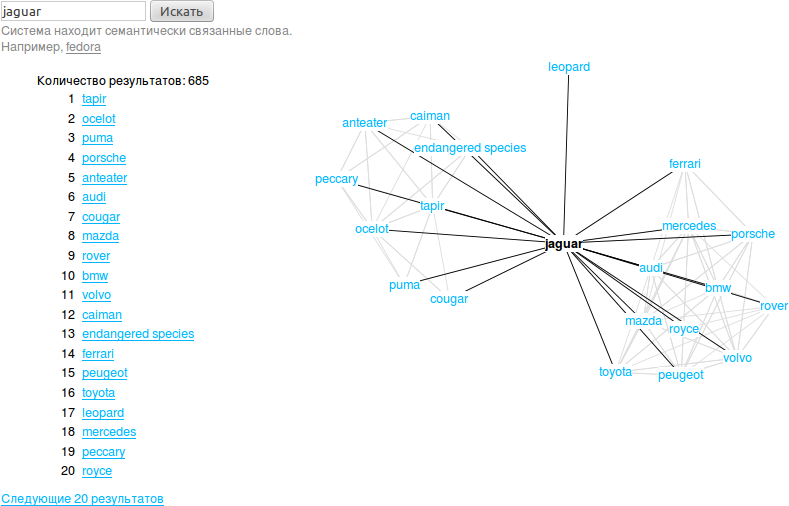
\includegraphics[width=0.9\textwidth]{jaguar}
\end{figure}

\end{frame}



\begin{frame}
\frametitle{Серелекс: результаты в виде множества изображений}

\includegraphics[width=1.0\textwidth]{./../figures/citroyen}

\end{frame}

\begin{frame}
\frametitle{Оценка качества работы системы Серелекс}

\begin{figure}
\center
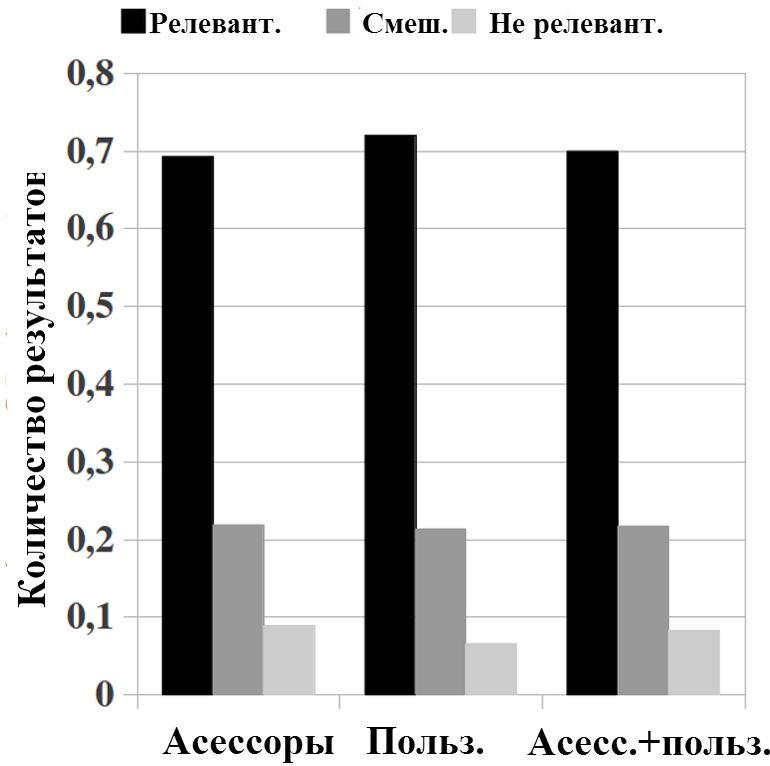
\includegraphics[width=0.5\textwidth]{serelex-eval}

\caption{Удовлетворенность пользователей первыми 20 результатами поиска для
594 запроса (23 ассесора и 109 пользователей).}
\end{figure}
\end{frame}


\subsection{Классификация коротких текстов}

\begin{frame}[fragile]
\frametitle{iCop: классификация имен файлов}

\begin{figure}
\center
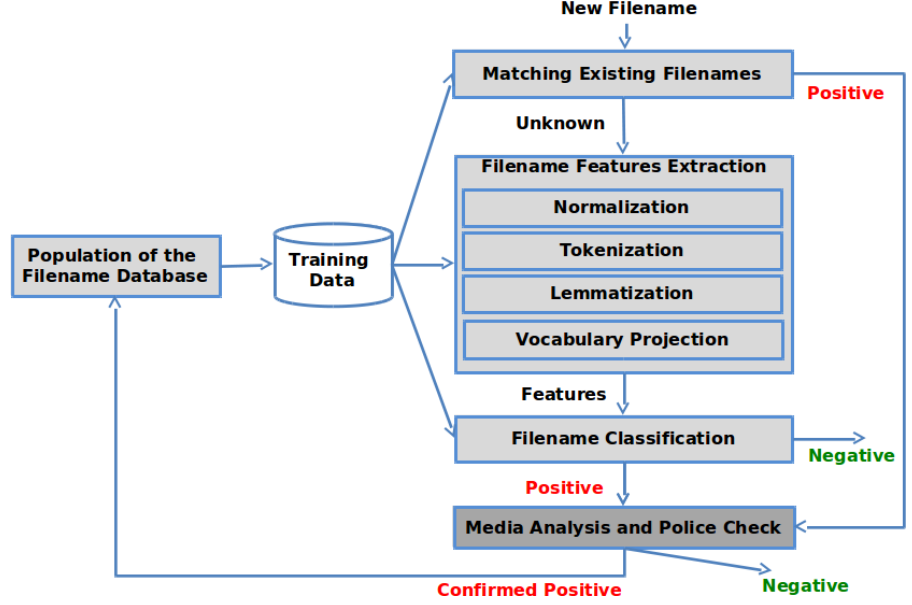
\includegraphics[width=0.7\textwidth]{./icop}
\caption{Структура системы.}
\end{figure}

\begin{itemize}
  \item Использование семантических отношений для расширения имени файла
  (Vocabulary Projection).
\end{itemize}


\end{frame}


\begin{frame}[fragile]
\frametitle{iCop: пример Vocabulary Projection}

\begin{figure}
\center
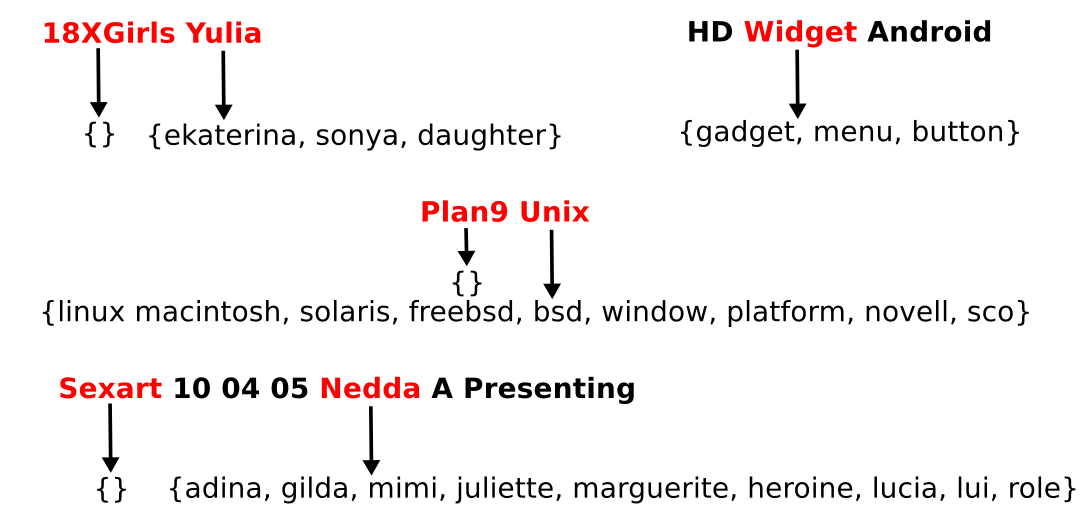
\includegraphics[width=0.9\textwidth]{./vp-ex}
\end{figure}



\end{frame}


\begin{frame}
\frametitle{Качество классификации}
\begin{table}
\tiny

%\footnotesize
\centering
\begin{tabular}{|l|l|l|l|}

\hline
\bf Обучающая выборка & \bf Тестовая выборка & \bf Accuracy  &
\textbf{Accuracy (voc. projection)} \\ \hline

Gallery (train) & Gallery  & 96.41 & \textbf{96.83} (+0.42) \\
PirateBay Title+Desc+Tags & PirateBay Title+Desc+Tags &  \textbf{98.92} &  98.86 (--0.06)\\
PirateBay Title+Tags & PirateBay Title+Tags & \textbf{97.73} & 97.63 (--0.10) \\
Gallery & PirateBay Title+Desc+Tags & 90.57 & \textbf{91.48} (+0.91) \\
\alert{Gallery}  & \alert{PirateBay Title+Tags}  & \alert{84.23} & \alert{\textbf{88.89}} \alert{(+4.66)} \\
PirateBay Title+Desc+Tags & Gallery  & 88.83 & \textbf{89.04} (+0.21) \\
PirateBay Title+Tags & Gallery & 91.16 & \textbf{91.30} (+0.14) \\
\hline

\end{tabular}
\caption{ Качество классификации с использованием C-SVM-linear c учетом
кросс-валидации.
}
\label{tbl:results2}

\end{table}
\end{frame}




%\section{Заключение}
%\subsection{}


%\begin{frame}
%\frametitle{The Key Contributions}

%### This dissertation explored several strategies to semantic relation extraction with similarity measures. 

% ### This work brings several contributions to the field of computational lexical semantics:

%\begin{enumerate}
%\item A corpus-based measure \textbf{SDA-MWE}: 
%\begin{itemize}
%\item performs comparably to the baselines;
%\item can deal with both single words and multiword expressions.
%\item was applied to automatic thesaurus construction.
%\end{itemize}

%\item A definition-based measure \textbf{DefVectors}:
%\begin{itemize}
%\item performs comparably to the baselines;
%\item operates on a small-scale set of definitions.
%\item an open source implemention.
%\end{itemize}
   
%\item A corpus-based measure \textbf{PatternSim}:
%\begin{itemize}
%\item performs comparably to the baseline measures;
%\item requires no semantic resources.
%\item an open source implemention.
%\end{itemize}

%\item A large-scale \textbf{comparative study} of the measures:
%\begin{itemize}
%\item comparison w.r.t. semantic relations provided by measures.
%\item evaluation scripts/datasets are available to the community.
%\end{itemize}


%\end{enumerate}

%\end{frame}

%\begin{frame}
%\frametitle{The Key Contributions (cont.)}

%\begin{enumerate}

%\setcounter{enumi}{4}



%\item Hybrid supervised semantic similarity measures \textbf{Logit-E15},
% \textbf{C-SVM-linear-E15}, \textbf{C-SVM-radial-E15}, etc.

%\begin{itemize}
 % \item based on the 5 types of resources;
 % \item outperforms baselines and other hybrid measures.

%\end{itemize}

%\item \textbf{Applications} which rely on the measure \textbf{PatternSim}:

%\begin{itemize}
%\item lexico-semantic search engine \textbf{Serelex};
%\begin{itemize}
%\item helps users discover similar words interactively;
%\item 70\% of users's satisfaction;
%\item an open source implementation.
%\end{itemize}

%\item Filename Categorization System system \textbf{iCOP}:
%\begin{itemize}
%\item categorizaton of file names;
%\item the measure refines accuracy of the baseline up to 5\%;
%\item an open source implementation. 
%\end{itemize}
% \end{itemize}

%\end{enumerate}

%\end{frame}





\begin{frame}
\frametitle{}

\Huge \bf Спасибо за внимание!

 \Huge \bf Вопросы?
\end{frame}
\end{document}